%% ------------------------------------------------------------------------- %%
\chapter{Introdução}
\label{cap:introducao}

Test-Driven Development (TDD) é uma das práticas mais populares da Programação
Extrema (XP) \cite{XPExplained}. 
Na opinião de muitos autores conhecidos, TDD agrega diversos benefícios ao
código produzido, dentre eles, simplicidade, foco, melhor design, entre outras.

Por esse motivo, é possível observar a crescente adoção e procura por TDD
através do número de pesquisas publicadas pela academia (muitas delas citadas no capítulo 
\ref{cap:trabalhos-relacionados}). Além disso, foi realizado o Primeiro Workshop
Internacional de Test-Driven Development em 2010, na cidade de Paris, organizado
pela Dra. Laurie Williams \footnote{http://agile.csc.ncsu.edu/tdd/. Último
acesso em 29/outubro/2010}.

Em um questionário de 2010, organizado por Scott Wambler, chamado de \textit{How
Agile Are You?} \cite{wambler-survey-agile}, mostra que 53\% dos times ágeis
adotaram TDD como uma maneira para validar o trabalho feito, conforme mostra a 
figura \ref{wambler-agile-2010}. Além disso, outro questionário de 2008, 
chamado de \textit{Test Driven Development (TDD) Survey}
\cite{wambler-survey-tdd}  mostra que 57\% dos desenvolvedores utilizam TDD como
técnica para capturar informações de design, conforme mostrado na figura 
\ref{wambler-tdd-2008}. 

No Brasil, é possível observar o crescente número de pessoas atrás de
informações sobre a prática nas mais diversas listas de discussão e fóruns sobre
tecnologia, como o GUJ \footnote{\url{http://www.guj.com.br}.
Último acesso em 27 de fevereiro 2011} ou o .NET Architects 
\footnote{\url{http://www.dotnetarchitects.net/}. Last access on February
27 de fevereiro de 2011}. Além disso, diversos eventos de desenvolvimento de
software realizados no Brasil em 2010, como a QCON SP
\footnote{\url{http://www.qconsp.com/}. Último acesso em 02 de março de 2011} e
a Agile Brazil \footnote{\url{http://http://www.agilebrazil.com/}. Último acesso
em 02 de março de 2011} contaram com palestras sobre o assunto.

Além disso, programadores que experimentam a prática e percebem seus
efeitos, raramente voltam atrás. Os aficionados por TDD dizem que estão
\textit{``infectados pelo teste''} \cite{tdd-fearless}.

Apesar de todos os possíveis vieses das informações apresentadas acima, os
números mostram que uma grande parte dos desenvolvedores ágeis já utilizam a 
prática no seu dia-a-dia.

\begin{figure}[h]
  \centering
  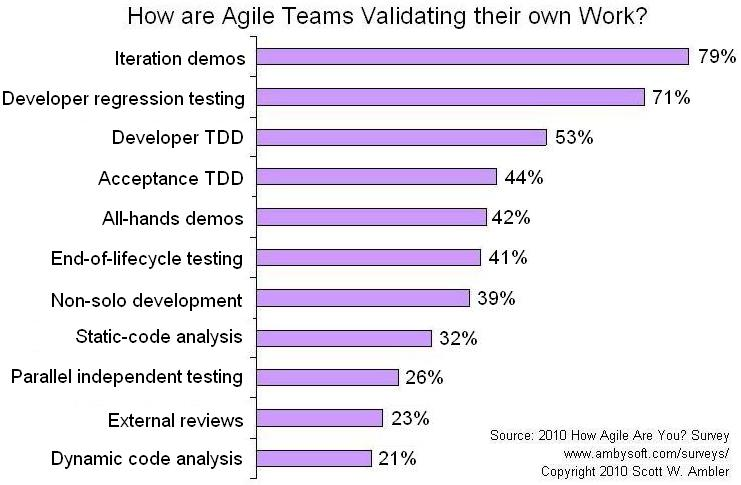
\includegraphics[scale=.6]{agileCriteria2010Validating}
  \caption{Como times ágeis validam seu próprio trabalho?}
  \label{fig:wambler-agile-2010}
\end{figure}

\begin{figure}[h]
  \centering
  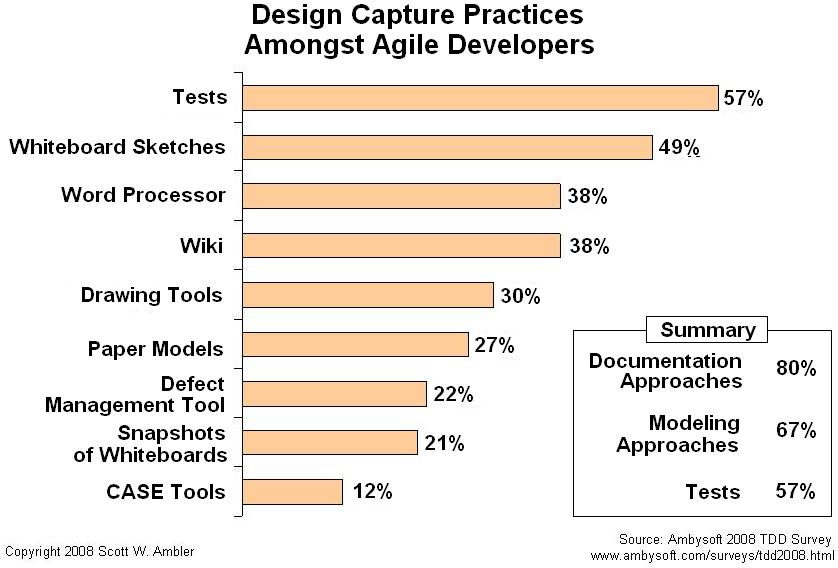
\includegraphics[scale=.5]{tddDesignPractices}
  \caption{Maneiras de captura de design entre desenvolvedores ágeis}   
  \label{fig:wambler-tdd-2008}
\end{figure}

Mas apesar da quantidade de programadores que adotam a prática, não é
fácil inverter a maneira de pensar; programadores estão acostumados a sempre
escrever os testes depois de escrever o código. Ao inverter o processo,
programadores são forçados a criar classes que apresentam um bom desenho.

É realmente difícil entender como TDD influencia no processo de desenvolvimento
de software. Apesar de ter o termo ``teste'' no nome, TDD é uma prática
de design. E, ao contrário do que se espera, boa parte dos experimentos da
academia sobre a prática verificam os efeitos dela sobre a qualidade externa. 

Poucos estudos avaliam TDD do ponto de vista da qualidade interna de código. E
além disso, Siniaalto e Abrahamsson notaram que os efeitos de TDD podem não ser
tão automáticos ou evidentes como o esperado \cite{alarming-results}.

Este trabalho visa compreender melhor os efeitos de prática de TDD sobre o
design de sistemas orientados a objetos do ponto de vista dos desenvolvedores
que a praticam. Para alcançar esse objetivo, esta pesquisa faz uso de métodos
qualitativos de pesquisa, melhor explicados no capítulo \ref{cap:planejamento}.

%% ------------------------------------------------------------------------- %%
\section{Contribuições}

O foco deste trabalho é entender de maneira mais profunda como TDD influencia no
design de sistemas orientados a objetos. Para alcançar esse objetivo, é necessário a
compreensão dos seguintes ítens:

\begin{itemize}
  \item Entender os efeitos de TDD sobre o acoplamento e coesão das classes
  criadas;

  \item Entender os efeitos de TDD sobre a simplicidade das classes criadas;

  \item Entender como o teste guia o desenvolvedor durante a atividade de
  design;

  \item Entender qual a relação entre a experiência do desenvolvedor com TDD e
  com sistemas orientados a objetos;
\end{itemize}
bla

%% ------------------------------------------------------------------------- %%
\section{Organização do trabalho}

Este trabalho é dividido da seguinte maneira: o capítulo \ref{cap:tdd} discute o
TDD sob o ponto de vista do design. O capítulo \ref{cap:design} apresenta boas
práticas e princípios de design que serão investigados durante o processo de
entrevistas. O capítulo \ref{cap:trabalhos-relacionados} mostra trabalhos já
realizados pela academia sobre os efeitos de TDD. Em seguida, o capítulo
\ref{cap:discussao} apresenta os resultados encontrados e discute em cima dos
mesmos. O capítulo \ref{cap:ameacas} discute as possíveis ameaças dos resultados
encontrados na pesquisa. E, por fim, o capítulo \ref{cap:conclusoes} resume o
trabalho realizado a apresenta possibilidades de trabalhos futuros.
